% Shared standalone design for the editable figure reconstructions.
\documentclass[tikz,border=5pt,10pt]{standalone}
\usepackage[T1]{fontenc}
\usepackage[utf8]{inputenc}
\usepackage{newpxtext,newpxmath}
\usepackage[scaled=.94]{sourcesanspro}
\usepackage{pgfplots}
\pgfplotsset{compat=1.18}
\usetikzlibrary{arrows.meta,calc,positioning,decorations.pathreplacing,
  decorations.markings,patterns,matrix,shapes.geometric,fit,backgrounds,
  intersections,angles,quotes}
\definecolor{ink}{HTML}{203746}
\definecolor{accent}{HTML}{146C78}
\definecolor{muted}{HTML}{667780}
\definecolor{signalred}{HTML}{B94B44}
\color{ink}
\tikzset{>=Latex,line width=.8pt,
  every node/.style={font=\small},
  axis/.style={->,draw=muted,line width=.5pt},
  guide/.style={draw=muted,dashed,line width=.45pt},
  curve/.style={draw=accent,line width=1pt},
  marker/.style={circle,fill=accent,inner sep=1.5pt},
  labelbox/.style={fill=white,inner sep=2pt}}

\begin{document}
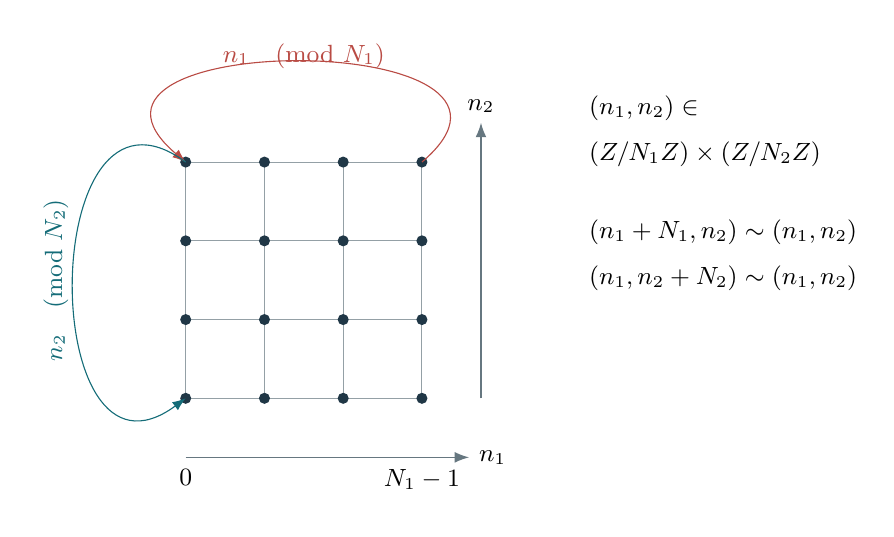
\begin{tikzpicture}[x=1cm,y=1cm]
\foreach \i in {0,1,2,3} {\draw[muted!70] (\i,0)--(\i,3) (0,\i)--(3,\i);}
\foreach \i in {0,1,2,3} {\foreach \j in {0,1,2,3} {\fill[ink] (\i,\j) circle(2pt);}}
\draw[->,signalred] (3,3)..controls(5,4.7)and(-2,4.7)..(0,3);
\draw[->,accent] (0,3)..controls(-1.9,4.4)and(-1.9,-1.4)..(0,0);
\node[signalred] at (1.5,4.35) {$n_1\pmod{N_1}$};
\node[accent,rotate=90] at (-1.65,1.5) {$n_2\pmod{N_2}$};
\draw[axis] (0,-.75)--(3.6,-.75) node[right] {$n_1$};
\draw[axis] (3.75,0)--(3.75,3.5) node[above] {$n_2$};
\node[below] at (0,-.78) {$0$};\node[below] at (3,-.78) {$N_1-1$};
\node[anchor=west,align=left] at (5,2.6) {$(n_1,n_2)\in$\\[2mm]$(\mathbb Z/N_1\mathbb Z)\times(\mathbb Z/N_2\mathbb Z)$\\[6mm]$(n_1+N_1,n_2)\sim(n_1,n_2)$\\[2mm]$(n_1,n_2+N_2)\sim(n_1,n_2)$};
\end{tikzpicture}
\end{document}
